\documentclass[../thesis_main.tex]{subfiles}

\begin{document}

\doublespacing
\section{Data and Estimation Procedure}
\label{section:data}

\subsection{Data}

The data for our analysis are drawn from a longitudinal Chicago Public Schools administrative dataset for both students and teachers. The available data extends almost thirty years, but for the our main analysis I  focus on Freshman cohorts from the 2011-12 school year to the 2013-14 school year, and thus use data from school years 2010-2011 to 2017-18 in order to include information on both prior-achievement and postsecondary outcomes. This dataset is particularly strong as it provides a near-comprehensive summary of nearly every aspect of the problem under consideration. A full description of the data available can be found in Appendix~\ref{appendix:data}, but, in general, I  consider three levels of data:

\subsubsection{1. Student Level} 

The student level dataset contains information on every student enrolled at CPS in the time period under consideration, with one observation per student per year. These data form the base from which I  construct and characterize our analytic sample. It contains both 1) demographic data, consisting of information on a student's background, 2) academic records data, which contains informaiton on student's test scores, graduation stutus, and other markers of a students trajectory, and finally 3) post-secondary data, on student's college enrollment status. Together, this provides a very encompassing picture of student's educational experience at CPS and beyond, which I  use both to provide our controls and some of the long term outcomes for analysis. 

\subsubsection{2. Class Level}

The class level dataset details, for each student, all of the classes which they took in a given semester. The dataset also links students with information on the classes in which they were enrolled each semester. This provides both descriptive information about the class subject and level. In addition, this dataset provides both a unique teacher ID number for the instructor of the class, as well as information on the letter gradethe student received. Together, these represent the main components necessary for our estimation procedure. I convert the letter grades in this data to a numerical scale following CPS's convention, where an A is equivalent to four points, a B is equivalent to three points, and so on. 

\textit{Teacher Information.} The class level dataset also links each class to the unique teacher ID of the instructor for that course. 

\subsubsection{3. Teacher Level} 

Our final dataset is at the teacher level, containing descriptive and demographic information for each CPS teacher. As mentioned above, this dataset can be linked to the class level dataset by means of the teacher ID. Unfortuantely, this data is only rigorously maintained up to the 2011-12 school year, and so is mainly used for balance tests on years of data prior to our main analysis cohort, as is detailed in Section~\ref{section:tests}.

%%% To add/do(?): For CPS, however, the quality of teacher IDs is less rigorously maintained than that of students IDs. Thus, I  employ a fuzzy matching procedure to better link our teacher level data with the corresponding class level data. 

\subsubsection{Sample Construction}

%% TO ADD: APPENDIX ON SAMPLE CONSTRUCTION AND DECISION RULES
I construct our sample using the three datasets listed above. As stated above, I  limit our analysis to students from the freshman cohorts in school years 2010-2011 to 2013-2014. For the class level dataset, I  limit our sample to enrollments in mathematics and English classes. I apply a variety of filters to correct for underlying data in the errors and ensure I  have the data necessary for each teacher in the sample to accurately estimate a grade effect. A full description of this procedure can be found in Appendix~\ref{appendix:data}, but in all, we arrive at an analytic sample consisting of one observation per student/subject pair, recorded over both freshman and sophmore year. 

%TODO: add reading, or social studies%.
%% TODO: ADD FILTERS FOR NUMBER OF TEACHERS A STUDENT SEES/NUMBER OF STUDENTS A TEACHER SEES? SEE GILRAINE

%% THIS WILL NEED TO BE CHANGED WHEN WE ADD MORE YEARS, ALSO CHECK LATER AFTER RERUNNING TABLES.
%% TODO: Add Apendix A table comapring cohort to main years. 

Table~\ref{tab:table_demographics} displays summary statistics for the analytic sample of the demographic variables described above, by freshman cohort. As this table shows, our analytic 2013-14 freshman cohort contains 11,125 observations. Over 80\% of these observations are students of color, which is relatively representative of CPS as a whole.

% TODO: Add real ref label to table, as well as fixing year. Also, should drop missing, soooo... do that. THIS TABLE NEEDS R WORK.

  \providecommand{\huxb}[2]{\arrayrulecolor[RGB]{#1}\global\arrayrulewidth=#2pt}
  \providecommand{\huxvb}[2]{\color[RGB]{#1}\vrule width #2pt}
  \providecommand{\huxtpad}[1]{\rule{0pt}{#1}}
  \providecommand{\huxbpad}[1]{\rule[-#1]{0pt}{#1}}

\begin{table}[h!]
\begin{centerbox}
\begin{threeparttable}
\captionsetup{justification=centering,singlelinecheck=off}
\caption{Demographics by Freshman Cohort}
 \label{tab:table_demographics}
\setlength{\tabcolsep}{0pt}
\begin{tabular}{l l l l l l}


\hhline{}
\arrayrulecolor{black}

\multicolumn{1}{!{\huxvb{0, 0, 0}{0}}l!{\huxvb{0, 0, 0}{0}}}{\huxtpad{6pt + 1em}\raggedright \hspace{6pt} Characteristic \hspace{6pt}\huxbpad{6pt}} &
\multicolumn{1}{c!{\huxvb{0, 0, 0}{0}}}{\huxtpad{6pt + 1em}\centering \hspace{6pt} 2010, N = 5,267 \hspace{6pt}\huxbpad{6pt}} &
\multicolumn{1}{c!{\huxvb{0, 0, 0}{0}}}{\huxtpad{6pt + 1em}\centering \hspace{6pt} 2011, N = 10,869 \hspace{6pt}\huxbpad{6pt}} &
\multicolumn{1}{c!{\huxvb{0, 0, 0}{0}}}{\huxtpad{6pt + 1em}\centering \hspace{6pt} 2012, N = 10,662 \hspace{6pt}\huxbpad{6pt}} &
\multicolumn{1}{c!{\huxvb{0, 0, 0}{0}}}{\huxtpad{6pt + 1em}\centering \hspace{6pt} 2013, N = 10,603 \hspace{6pt}\huxbpad{6pt}} &
\multicolumn{1}{c!{\huxvb{0, 0, 0}{0}}}{\huxtpad{6pt + 1em}\centering \hspace{6pt} 2014, N = 9,445 \hspace{6pt}\huxbpad{6pt}} \tabularnewline[-0.5pt]


\hhline{>{\huxb{0, 0, 0}{0.4}}->{\huxb{0, 0, 0}{0.4}}->{\huxb{0, 0, 0}{0.4}}->{\huxb{0, 0, 0}{0.4}}->{\huxb{0, 0, 0}{0.4}}->{\huxb{0, 0, 0}{0.4}}-}
\arrayrulecolor{black}

\multicolumn{1}{!{\huxvb{0, 0, 0}{0}}l!{\huxvb{0, 0, 0}{0}}}{\huxtpad{6pt + 1em}\raggedright \hspace{6pt} Race \hspace{6pt}\huxbpad{6pt}} &
\multicolumn{1}{c!{\huxvb{0, 0, 0}{0}}}{\huxtpad{6pt + 1em}\centering \hspace{6pt}  \hspace{6pt}\huxbpad{6pt}} &
\multicolumn{1}{c!{\huxvb{0, 0, 0}{0}}}{\huxtpad{6pt + 1em}\centering \hspace{6pt}  \hspace{6pt}\huxbpad{6pt}} &
\multicolumn{1}{c!{\huxvb{0, 0, 0}{0}}}{\huxtpad{6pt + 1em}\centering \hspace{6pt}  \hspace{6pt}\huxbpad{6pt}} &
\multicolumn{1}{c!{\huxvb{0, 0, 0}{0}}}{\huxtpad{6pt + 1em}\centering \hspace{6pt}  \hspace{6pt}\huxbpad{6pt}} &
\multicolumn{1}{c!{\huxvb{0, 0, 0}{0}}}{\huxtpad{6pt + 1em}\centering \hspace{6pt}  \hspace{6pt}\huxbpad{6pt}} \tabularnewline[-0.5pt]


\hhline{}
\arrayrulecolor{black}

\multicolumn{1}{!{\huxvb{0, 0, 0}{0}}l!{\huxvb{0, 0, 0}{0}}}{\huxtpad{6pt + 1em}\raggedright \hspace{15pt} Latino \hspace{6pt}\huxbpad{6pt}} &
\multicolumn{1}{c!{\huxvb{0, 0, 0}{0}}}{\huxtpad{6pt + 1em}\centering \hspace{6pt} 2,660 (51\%) \hspace{6pt}\huxbpad{6pt}} &
\multicolumn{1}{c!{\huxvb{0, 0, 0}{0}}}{\huxtpad{6pt + 1em}\centering \hspace{6pt} 5,460 (50\%) \hspace{6pt}\huxbpad{6pt}} &
\multicolumn{1}{c!{\huxvb{0, 0, 0}{0}}}{\huxtpad{6pt + 1em}\centering \hspace{6pt} 5,595 (52\%) \hspace{6pt}\huxbpad{6pt}} &
\multicolumn{1}{c!{\huxvb{0, 0, 0}{0}}}{\huxtpad{6pt + 1em}\centering \hspace{6pt} 5,539 (52\%) \hspace{6pt}\huxbpad{6pt}} &
\multicolumn{1}{c!{\huxvb{0, 0, 0}{0}}}{\huxtpad{6pt + 1em}\centering \hspace{6pt} 5,013 (53\%) \hspace{6pt}\huxbpad{6pt}} \tabularnewline[-0.5pt]


\hhline{}
\arrayrulecolor{black}

\multicolumn{1}{!{\huxvb{0, 0, 0}{0}}l!{\huxvb{0, 0, 0}{0}}}{\huxtpad{6pt + 1em}\raggedright \hspace{15pt} Black \hspace{6pt}\huxbpad{6pt}} &
\multicolumn{1}{c!{\huxvb{0, 0, 0}{0}}}{\huxtpad{6pt + 1em}\centering \hspace{6pt} 1,725 (33\%) \hspace{6pt}\huxbpad{6pt}} &
\multicolumn{1}{c!{\huxvb{0, 0, 0}{0}}}{\huxtpad{6pt + 1em}\centering \hspace{6pt} 3,406 (31\%) \hspace{6pt}\huxbpad{6pt}} &
\multicolumn{1}{c!{\huxvb{0, 0, 0}{0}}}{\huxtpad{6pt + 1em}\centering \hspace{6pt} 3,193 (30\%) \hspace{6pt}\huxbpad{6pt}} &
\multicolumn{1}{c!{\huxvb{0, 0, 0}{0}}}{\huxtpad{6pt + 1em}\centering \hspace{6pt} 3,068 (29\%) \hspace{6pt}\huxbpad{6pt}} &
\multicolumn{1}{c!{\huxvb{0, 0, 0}{0}}}{\huxtpad{6pt + 1em}\centering \hspace{6pt} 2,584 (27\%) \hspace{6pt}\huxbpad{6pt}} \tabularnewline[-0.5pt]


\hhline{}
\arrayrulecolor{black}

\multicolumn{1}{!{\huxvb{0, 0, 0}{0}}l!{\huxvb{0, 0, 0}{0}}}{\huxtpad{6pt + 1em}\raggedright \hspace{15pt} White \hspace{6pt}\huxbpad{6pt}} &
\multicolumn{1}{c!{\huxvb{0, 0, 0}{0}}}{\huxtpad{6pt + 1em}\centering \hspace{6pt} 491 (9.3\%) \hspace{6pt}\huxbpad{6pt}} &
\multicolumn{1}{c!{\huxvb{0, 0, 0}{0}}}{\huxtpad{6pt + 1em}\centering \hspace{6pt} 1,173 (11\%) \hspace{6pt}\huxbpad{6pt}} &
\multicolumn{1}{c!{\huxvb{0, 0, 0}{0}}}{\huxtpad{6pt + 1em}\centering \hspace{6pt} 1,098 (10\%) \hspace{6pt}\huxbpad{6pt}} &
\multicolumn{1}{c!{\huxvb{0, 0, 0}{0}}}{\huxtpad{6pt + 1em}\centering \hspace{6pt} 1,164 (11\%) \hspace{6pt}\huxbpad{6pt}} &
\multicolumn{1}{c!{\huxvb{0, 0, 0}{0}}}{\huxtpad{6pt + 1em}\centering \hspace{6pt} 1,074 (11\%) \hspace{6pt}\huxbpad{6pt}} \tabularnewline[-0.5pt]


\hhline{}
\arrayrulecolor{black}

\multicolumn{1}{!{\huxvb{0, 0, 0}{0}}l!{\huxvb{0, 0, 0}{0}}}{\huxtpad{6pt + 1em}\raggedright \hspace{15pt} Asian \hspace{6pt}\huxbpad{6pt}} &
\multicolumn{1}{c!{\huxvb{0, 0, 0}{0}}}{\huxtpad{6pt + 1em}\centering \hspace{6pt} 304 (5.8\%) \hspace{6pt}\huxbpad{6pt}} &
\multicolumn{1}{c!{\huxvb{0, 0, 0}{0}}}{\huxtpad{6pt + 1em}\centering \hspace{6pt} 638 (5.9\%) \hspace{6pt}\huxbpad{6pt}} &
\multicolumn{1}{c!{\huxvb{0, 0, 0}{0}}}{\huxtpad{6pt + 1em}\centering \hspace{6pt} 614 (5.8\%) \hspace{6pt}\huxbpad{6pt}} &
\multicolumn{1}{c!{\huxvb{0, 0, 0}{0}}}{\huxtpad{6pt + 1em}\centering \hspace{6pt} 666 (6.3\%) \hspace{6pt}\huxbpad{6pt}} &
\multicolumn{1}{c!{\huxvb{0, 0, 0}{0}}}{\huxtpad{6pt + 1em}\centering \hspace{6pt} 605 (6.4\%) \hspace{6pt}\huxbpad{6pt}} \tabularnewline[-0.5pt]


\hhline{}
\arrayrulecolor{black}

\multicolumn{1}{!{\huxvb{0, 0, 0}{0}}l!{\huxvb{0, 0, 0}{0}}}{\huxtpad{6pt + 1em}\raggedright \hspace{15pt} Multiracial \hspace{6pt}\huxbpad{6pt}} &
\multicolumn{1}{c!{\huxvb{0, 0, 0}{0}}}{\huxtpad{6pt + 1em}\centering \hspace{6pt} 60 (1.1\%) \hspace{6pt}\huxbpad{6pt}} &
\multicolumn{1}{c!{\huxvb{0, 0, 0}{0}}}{\huxtpad{6pt + 1em}\centering \hspace{6pt} 148 (1.4\%) \hspace{6pt}\huxbpad{6pt}} &
\multicolumn{1}{c!{\huxvb{0, 0, 0}{0}}}{\huxtpad{6pt + 1em}\centering \hspace{6pt} 119 (1.1\%) \hspace{6pt}\huxbpad{6pt}} &
\multicolumn{1}{c!{\huxvb{0, 0, 0}{0}}}{\huxtpad{6pt + 1em}\centering \hspace{6pt} 126 (1.2\%) \hspace{6pt}\huxbpad{6pt}} &
\multicolumn{1}{c!{\huxvb{0, 0, 0}{0}}}{\huxtpad{6pt + 1em}\centering \hspace{6pt} 125 (1.3\%) \hspace{6pt}\huxbpad{6pt}} \tabularnewline[-0.5pt]


\hhline{}
\arrayrulecolor{black}

\multicolumn{1}{!{\huxvb{0, 0, 0}{0}}l!{\huxvb{0, 0, 0}{0}}}{\huxtpad{6pt + 1em}\raggedright \hspace{15pt} Other \hspace{6pt}\huxbpad{6pt}} &
\multicolumn{1}{c!{\huxvb{0, 0, 0}{0}}}{\huxtpad{6pt + 1em}\centering \hspace{6pt} 27 (0.5\%) \hspace{6pt}\huxbpad{6pt}} &
\multicolumn{1}{c!{\huxvb{0, 0, 0}{0}}}{\huxtpad{6pt + 1em}\centering \hspace{6pt} 43 (0.4\%) \hspace{6pt}\huxbpad{6pt}} &
\multicolumn{1}{c!{\huxvb{0, 0, 0}{0}}}{\huxtpad{6pt + 1em}\centering \hspace{6pt} 40 (0.4\%) \hspace{6pt}\huxbpad{6pt}} &
\multicolumn{1}{c!{\huxvb{0, 0, 0}{0}}}{\huxtpad{6pt + 1em}\centering \hspace{6pt} 37 (0.3\%) \hspace{6pt}\huxbpad{6pt}} &
\multicolumn{1}{c!{\huxvb{0, 0, 0}{0}}}{\huxtpad{6pt + 1em}\centering \hspace{6pt} 42 (0.4\%) \hspace{6pt}\huxbpad{6pt}} \tabularnewline[-0.5pt]


\hhline{}
\arrayrulecolor{black}

\multicolumn{1}{!{\huxvb{0, 0, 0}{0}}l!{\huxvb{0, 0, 0}{0}}}{\huxtpad{6pt + 1em}\raggedright \hspace{15pt} Unknown Race/Ethnicity \hspace{6pt}\huxbpad{6pt}} &
\multicolumn{1}{c!{\huxvb{0, 0, 0}{0}}}{\huxtpad{6pt + 1em}\centering \hspace{6pt} 0 (0\%) \hspace{6pt}\huxbpad{6pt}} &
\multicolumn{1}{c!{\huxvb{0, 0, 0}{0}}}{\huxtpad{6pt + 1em}\centering \hspace{6pt} 1 ($<$0.1\%) \hspace{6pt}\huxbpad{6pt}} &
\multicolumn{1}{c!{\huxvb{0, 0, 0}{0}}}{\huxtpad{6pt + 1em}\centering \hspace{6pt} 3 ($<$0.1\%) \hspace{6pt}\huxbpad{6pt}} &
\multicolumn{1}{c!{\huxvb{0, 0, 0}{0}}}{\huxtpad{6pt + 1em}\centering \hspace{6pt} 3 ($<$0.1\%) \hspace{6pt}\huxbpad{6pt}} &
\multicolumn{1}{c!{\huxvb{0, 0, 0}{0}}}{\huxtpad{6pt + 1em}\centering \hspace{6pt} 2 ($<$0.1\%) \hspace{6pt}\huxbpad{6pt}} \tabularnewline[-0.5pt]


\hhline{}
\arrayrulecolor{black}

\multicolumn{1}{!{\huxvb{0, 0, 0}{0}}l!{\huxvb{0, 0, 0}{0}}}{\huxtpad{6pt + 1em}\raggedright \hspace{6pt} Gender \hspace{6pt}\huxbpad{6pt}} &
\multicolumn{1}{c!{\huxvb{0, 0, 0}{0}}}{\huxtpad{6pt + 1em}\centering \hspace{6pt}  \hspace{6pt}\huxbpad{6pt}} &
\multicolumn{1}{c!{\huxvb{0, 0, 0}{0}}}{\huxtpad{6pt + 1em}\centering \hspace{6pt}  \hspace{6pt}\huxbpad{6pt}} &
\multicolumn{1}{c!{\huxvb{0, 0, 0}{0}}}{\huxtpad{6pt + 1em}\centering \hspace{6pt}  \hspace{6pt}\huxbpad{6pt}} &
\multicolumn{1}{c!{\huxvb{0, 0, 0}{0}}}{\huxtpad{6pt + 1em}\centering \hspace{6pt}  \hspace{6pt}\huxbpad{6pt}} &
\multicolumn{1}{c!{\huxvb{0, 0, 0}{0}}}{\huxtpad{6pt + 1em}\centering \hspace{6pt}  \hspace{6pt}\huxbpad{6pt}} \tabularnewline[-0.5pt]


\hhline{}
\arrayrulecolor{black}

\multicolumn{1}{!{\huxvb{0, 0, 0}{0}}l!{\huxvb{0, 0, 0}{0}}}{\huxtpad{6pt + 1em}\raggedright \hspace{15pt} Female \hspace{6pt}\huxbpad{6pt}} &
\multicolumn{1}{c!{\huxvb{0, 0, 0}{0}}}{\huxtpad{6pt + 1em}\centering \hspace{6pt} 2,847 (54\%) \hspace{6pt}\huxbpad{6pt}} &
\multicolumn{1}{c!{\huxvb{0, 0, 0}{0}}}{\huxtpad{6pt + 1em}\centering \hspace{6pt} 5,959 (55\%) \hspace{6pt}\huxbpad{6pt}} &
\multicolumn{1}{c!{\huxvb{0, 0, 0}{0}}}{\huxtpad{6pt + 1em}\centering \hspace{6pt} 5,877 (55\%) \hspace{6pt}\huxbpad{6pt}} &
\multicolumn{1}{c!{\huxvb{0, 0, 0}{0}}}{\huxtpad{6pt + 1em}\centering \hspace{6pt} 5,842 (55\%) \hspace{6pt}\huxbpad{6pt}} &
\multicolumn{1}{c!{\huxvb{0, 0, 0}{0}}}{\huxtpad{6pt + 1em}\centering \hspace{6pt} 5,200 (55\%) \hspace{6pt}\huxbpad{6pt}} \tabularnewline[-0.5pt]


\hhline{}
\arrayrulecolor{black}

\multicolumn{1}{!{\huxvb{0, 0, 0}{0}}l!{\huxvb{0, 0, 0}{0}}}{\huxtpad{6pt + 1em}\raggedright \hspace{15pt} Male \hspace{6pt}\huxbpad{6pt}} &
\multicolumn{1}{c!{\huxvb{0, 0, 0}{0}}}{\huxtpad{6pt + 1em}\centering \hspace{6pt} 2,420 (46\%) \hspace{6pt}\huxbpad{6pt}} &
\multicolumn{1}{c!{\huxvb{0, 0, 0}{0}}}{\huxtpad{6pt + 1em}\centering \hspace{6pt} 4,910 (45\%) \hspace{6pt}\huxbpad{6pt}} &
\multicolumn{1}{c!{\huxvb{0, 0, 0}{0}}}{\huxtpad{6pt + 1em}\centering \hspace{6pt} 4,785 (45\%) \hspace{6pt}\huxbpad{6pt}} &
\multicolumn{1}{c!{\huxvb{0, 0, 0}{0}}}{\huxtpad{6pt + 1em}\centering \hspace{6pt} 4,761 (45\%) \hspace{6pt}\huxbpad{6pt}} &
\multicolumn{1}{c!{\huxvb{0, 0, 0}{0}}}{\huxtpad{6pt + 1em}\centering \hspace{6pt} 4,245 (45\%) \hspace{6pt}\huxbpad{6pt}} \tabularnewline[-0.5pt]


\hhline{}
\arrayrulecolor{black}

\multicolumn{1}{!{\huxvb{0, 0, 0}{0}}l!{\huxvb{0, 0, 0}{0}}}{\huxtpad{6pt + 1em}\raggedright \hspace{6pt} Census Block - \% Families Below Poverty \hspace{6pt}\huxbpad{6pt}} &
\multicolumn{1}{c!{\huxvb{0, 0, 0}{0}}}{\huxtpad{6pt + 1em}\centering \hspace{6pt} 21.24 (15.67) \hspace{6pt}\huxbpad{6pt}} &
\multicolumn{1}{c!{\huxvb{0, 0, 0}{0}}}{\huxtpad{6pt + 1em}\centering \hspace{6pt} 20.71 (15.79) \hspace{6pt}\huxbpad{6pt}} &
\multicolumn{1}{c!{\huxvb{0, 0, 0}{0}}}{\huxtpad{6pt + 1em}\centering \hspace{6pt} 20.39 (15.57) \hspace{6pt}\huxbpad{6pt}} &
\multicolumn{1}{c!{\huxvb{0, 0, 0}{0}}}{\huxtpad{6pt + 1em}\centering \hspace{6pt} 20.42 (15.39) \hspace{6pt}\huxbpad{6pt}} &
\multicolumn{1}{c!{\huxvb{0, 0, 0}{0}}}{\huxtpad{6pt + 1em}\centering \hspace{6pt} 19.99 (15.27) \hspace{6pt}\huxbpad{6pt}} \tabularnewline[-0.5pt]


\hhline{}
\arrayrulecolor{black}

\multicolumn{1}{!{\huxvb{0, 0, 0}{0}}l!{\huxvb{0, 0, 0}{0}}}{\huxtpad{6pt + 1em}\raggedright \hspace{6pt} Age at Start of Freshmen Year \hspace{6pt}\huxbpad{6pt}} &
\multicolumn{1}{c!{\huxvb{0, 0, 0}{0}}}{\huxtpad{6pt + 1em}\centering \hspace{6pt} 14.09 (0.33) \hspace{6pt}\huxbpad{6pt}} &
\multicolumn{1}{c!{\huxvb{0, 0, 0}{0}}}{\huxtpad{6pt + 1em}\centering \hspace{6pt} 14.09 (0.35) \hspace{6pt}\huxbpad{6pt}} &
\multicolumn{1}{c!{\huxvb{0, 0, 0}{0}}}{\huxtpad{6pt + 1em}\centering \hspace{6pt} 14.07 (0.32) \hspace{6pt}\huxbpad{6pt}} &
\multicolumn{1}{c!{\huxvb{0, 0, 0}{0}}}{\huxtpad{6pt + 1em}\centering \hspace{6pt} 14.07 (0.33) \hspace{6pt}\huxbpad{6pt}} &
\multicolumn{1}{c!{\huxvb{0, 0, 0}{0}}}{\huxtpad{6pt + 1em}\centering \hspace{6pt} 14.06 (0.29) \hspace{6pt}\huxbpad{6pt}} \tabularnewline[-0.5pt]


\hhline{>{\huxb{0, 0, 0}{0.8}}->{\huxb{0, 0, 0}{0.8}}->{\huxb{0, 0, 0}{0.8}}->{\huxb{0, 0, 0}{0.8}}->{\huxb{0, 0, 0}{0.8}}->{\huxb{0, 0, 0}{0.8}}-}
\arrayrulecolor{black}

\multicolumn{6}{!{\huxvb{0, 0, 0}{0}}l!{\huxvb{0, 0, 0}{0}}}{\huxtpad{6pt + 1em}\raggedright \hspace{6pt} n (\%); Mean (SD) \hspace{6pt}\huxbpad{6pt}} \tabularnewline[-0.5pt]


\hhline{}
\arrayrulecolor{black}
\end{tabular}
\end{threeparttable}\par\end{centerbox}

\end{table}


% TODO: add real ref label to table. THIS TABLE NEEDS R WORK. ALSO FIX YEAR. WHY ARE MATH AND READING Z SCORES NOT STANDARDIZED. 
%% TODO: Add 8th grade GPA?

Similarly, Table~\ref{tab:table_eigth_grade} displays summary statistics for the eighth grade prior achievement variables for our analytic sample. The first two row contain information on the standardized eighth grade math and reading scores for students in our sample. These scores are standardized at the full cohort level to have mean zero and variance one. The fact that the mean scores within our cohort are slightly higher than zero in each case therefore represents a slight positive selection effect of our sample. This same positive biasis widely observed across the literature, and is highlighted in \citet{gilraineMakingTeachingLast2020}. In our case, it likely results from dropping students with missing grade data, who may be in alternative schools or programs and, on the whole, slightly under-performing. A similar bias is observed within the eighth grade attendance, grade, and discipline variables.


  \providecommand{\huxb}[2]{\arrayrulecolor[RGB]{#1}\global\arrayrulewidth=#2pt}
  \providecommand{\huxvb}[2]{\color[RGB]{#1}\vrule width #2pt}
  \providecommand{\huxtpad}[1]{\rule{0pt}{#1}}
  \providecommand{\huxbpad}[1]{\rule[-#1]{0pt}{#1}}

\begin{table}[h!]
\begin{centerbox}
\begin{threeparttable}
\captionsetup{justification=centering,singlelinecheck=off}
\caption{8th Grade Outcomes by Cohorts}
 \label{tab:table_eigth_grade}
\setlength{\tabcolsep}{0pt}
\begin{tabular}{l l l l}


\hhline{}
\arrayrulecolor{black}

\multicolumn{1}{!{\huxvb{0, 0, 0}{0}}l!{\huxvb{0, 0, 0}{0}}}{\huxtpad{6pt + 1em}\raggedright \hspace{6pt} Outcome \hspace{6pt}\huxbpad{6pt}} &
\multicolumn{1}{c!{\huxvb{0, 0, 0}{0}}}{\huxtpad{6pt + 1em}\centering \hspace{6pt} 2011, N = 14,389 \hspace{6pt}\huxbpad{6pt}} &
\multicolumn{1}{c!{\huxvb{0, 0, 0}{0}}}{\huxtpad{6pt + 1em}\centering \hspace{6pt} 2012, N = 13,602 \hspace{6pt}\huxbpad{6pt}} &
\multicolumn{1}{c!{\huxvb{0, 0, 0}{0}}}{\huxtpad{6pt + 1em}\centering \hspace{6pt} 2013, N = 12,954 \hspace{6pt}\huxbpad{6pt}} \tabularnewline[-0.5pt]


\hhline{>{\huxb{0, 0, 0}{0.4}}->{\huxb{0, 0, 0}{0.4}}->{\huxb{0, 0, 0}{0.4}}->{\huxb{0, 0, 0}{0.4}}-}
\arrayrulecolor{black}

\multicolumn{1}{!{\huxvb{0, 0, 0}{0}}l!{\huxvb{0, 0, 0}{0}}}{\huxtpad{6pt + 1em}\raggedright \hspace{6pt} 8th Grade Math Score (Standardized) \hspace{6pt}\huxbpad{6pt}} &
\multicolumn{1}{c!{\huxvb{0, 0, 0}{0}}}{\huxtpad{6pt + 1em}\centering \hspace{6pt} 0.2423 (1.0150) \hspace{6pt}\huxbpad{6pt}} &
\multicolumn{1}{c!{\huxvb{0, 0, 0}{0}}}{\huxtpad{6pt + 1em}\centering \hspace{6pt} 0.2581 (1.0182) \hspace{6pt}\huxbpad{6pt}} &
\multicolumn{1}{c!{\huxvb{0, 0, 0}{0}}}{\huxtpad{6pt + 1em}\centering \hspace{6pt} 0.2788 (1.0236) \hspace{6pt}\huxbpad{6pt}} \tabularnewline[-0.5pt]


\hhline{}
\arrayrulecolor{black}

\multicolumn{1}{!{\huxvb{0, 0, 0}{0}}l!{\huxvb{0, 0, 0}{0}}}{\huxtpad{6pt + 1em}\raggedright \hspace{6pt} 8th Grade Reading Score (Standardized) \hspace{6pt}\huxbpad{6pt}} &
\multicolumn{1}{c!{\huxvb{0, 0, 0}{0}}}{\huxtpad{6pt + 1em}\centering \hspace{6pt} 0.2213 (0.9242) \hspace{6pt}\huxbpad{6pt}} &
\multicolumn{1}{c!{\huxvb{0, 0, 0}{0}}}{\huxtpad{6pt + 1em}\centering \hspace{6pt} 0.2471 (0.9383) \hspace{6pt}\huxbpad{6pt}} &
\multicolumn{1}{c!{\huxvb{0, 0, 0}{0}}}{\huxtpad{6pt + 1em}\centering \hspace{6pt} 0.2477 (0.9495) \hspace{6pt}\huxbpad{6pt}} \tabularnewline[-0.5pt]


\hhline{}
\arrayrulecolor{black}

\multicolumn{1}{!{\huxvb{0, 0, 0}{0}}l!{\huxvb{0, 0, 0}{0}}}{\huxtpad{6pt + 1em}\raggedright \hspace{6pt} 8th Grade Core GPA \hspace{6pt}\huxbpad{6pt}} &
\multicolumn{1}{c!{\huxvb{0, 0, 0}{0}}}{\huxtpad{6pt + 1em}\centering \hspace{6pt} 2.6702 (0.8886) \hspace{6pt}\huxbpad{6pt}} &
\multicolumn{1}{c!{\huxvb{0, 0, 0}{0}}}{\huxtpad{6pt + 1em}\centering \hspace{6pt} 2.7298 (0.8654) \hspace{6pt}\huxbpad{6pt}} &
\multicolumn{1}{c!{\huxvb{0, 0, 0}{0}}}{\huxtpad{6pt + 1em}\centering \hspace{6pt} 2.8015 (0.8535) \hspace{6pt}\huxbpad{6pt}} \tabularnewline[-0.5pt]


\hhline{}
\arrayrulecolor{black}

\multicolumn{1}{!{\huxvb{0, 0, 0}{0}}l!{\huxvb{0, 0, 0}{0}}}{\huxtpad{6pt + 1em}\raggedright \hspace{6pt} 8th Grade Attendance (Fraction of Days Attended) \hspace{6pt}\huxbpad{6pt}} &
\multicolumn{1}{c!{\huxvb{0, 0, 0}{0}}}{\huxtpad{6pt + 1em}\centering \hspace{6pt} 0.9560 (0.0450) \hspace{6pt}\huxbpad{6pt}} &
\multicolumn{1}{c!{\huxvb{0, 0, 0}{0}}}{\huxtpad{6pt + 1em}\centering \hspace{6pt} 0.9600 (0.0429) \hspace{6pt}\huxbpad{6pt}} &
\multicolumn{1}{c!{\huxvb{0, 0, 0}{0}}}{\huxtpad{6pt + 1em}\centering \hspace{6pt} 0.9507 (0.0446) \hspace{6pt}\huxbpad{6pt}} \tabularnewline[-0.5pt]


\hhline{}
\arrayrulecolor{black}

\multicolumn{1}{!{\huxvb{0, 0, 0}{0}}l!{\huxvb{0, 0, 0}{0}}}{\huxtpad{6pt + 1em}\raggedright \hspace{6pt} 8th Grade Discipline (no. of infractions) \hspace{6pt}\huxbpad{6pt}} &
\multicolumn{1}{c!{\huxvb{0, 0, 0}{0}}}{\huxtpad{6pt + 1em}\centering \hspace{6pt} 0.3080 (1.1064) \hspace{6pt}\huxbpad{6pt}} &
\multicolumn{1}{c!{\huxvb{0, 0, 0}{0}}}{\huxtpad{6pt + 1em}\centering \hspace{6pt} 0.2580 (0.9595) \hspace{6pt}\huxbpad{6pt}} &
\multicolumn{1}{c!{\huxvb{0, 0, 0}{0}}}{\huxtpad{6pt + 1em}\centering \hspace{6pt} 0.2877 (1.2475) \hspace{6pt}\huxbpad{6pt}} \tabularnewline[-0.5pt]


\hhline{>{\huxb{0, 0, 0}{0.8}}->{\huxb{0, 0, 0}{0.8}}->{\huxb{0, 0, 0}{0.8}}->{\huxb{0, 0, 0}{0.8}}-}
\arrayrulecolor{black}

\multicolumn{4}{!{\huxvb{0, 0, 0}{0}}l!{\huxvb{0, 0, 0}{0}}}{\huxtpad{6pt + 1em}\raggedright \hspace{6pt} Mean (SD) \hspace{6pt}\huxbpad{6pt}} \tabularnewline[-0.5pt]


\hhline{}
\arrayrulecolor{black}
\end{tabular}
\end{threeparttable}\par\end{centerbox}

\end{table}


Table~\ref{tab:table_freq} displays descriptives on the grades data for the analytic cohort, giving the number of students, teachers, and average grades by subject. In this analytic sample, there are slightly more observations of English grades than mathematics grades, but, within these observations, more unique math teachers than English teachers. I also see that, in this analytic sample, student's English grades are on average slightly higher than math grades, and display a lower standard deviation. This indicates some clustering at the upper end of English grades, while math grades have a more dispersed distribution.

\begin{table}

\caption{\label{tab:table_freq}Frequencies of Grade Variables by Freshman Cohort}
\centering
\begin{tabular}[t]{lr}
\toprule{}
  & 2013\\
\midrule{}
Number of Students & 11125\\
Number of Teachers & 1524\\
Number of Schools & 111\\
\addlinespace
Math Grades & 9752\\
Reading Grades & 10165\\
Social Studies Grades & 9265\\
Science Grades & 9530\\
\bottomrule{}
\end{tabular}
\end{table}


The final row of Table~\ref{tab:table_freq} average numerical difference between freshman and sophomore grades relatively low for both math and English classes, albeit with high variability for each. Some intuition behind this is given by Figure\ref{fig:grade_comp}. For a given freshman grade, this figure displays the percentage of students in our analytic sample who received each corresponding grade their sophomore year. The strong correlation down the diagonal axis represents exactly the same trend as the zero mean in the previous table: students often receive the same grade in their sophomore year class as they did previously in their freshman year class. This figure also shows, however, that this is in no way a guarantee, as there is still large amount of dispersion from this trend, with students both increasing and decreasing their grade between the two years. The proportion of this variability that is unexplained by observed factors is the primary variation used to identify our model. 

\begin{figure}[H]
	\centering
	\begin{subfigure}[b]{0.49\textwidth}
		\centering
		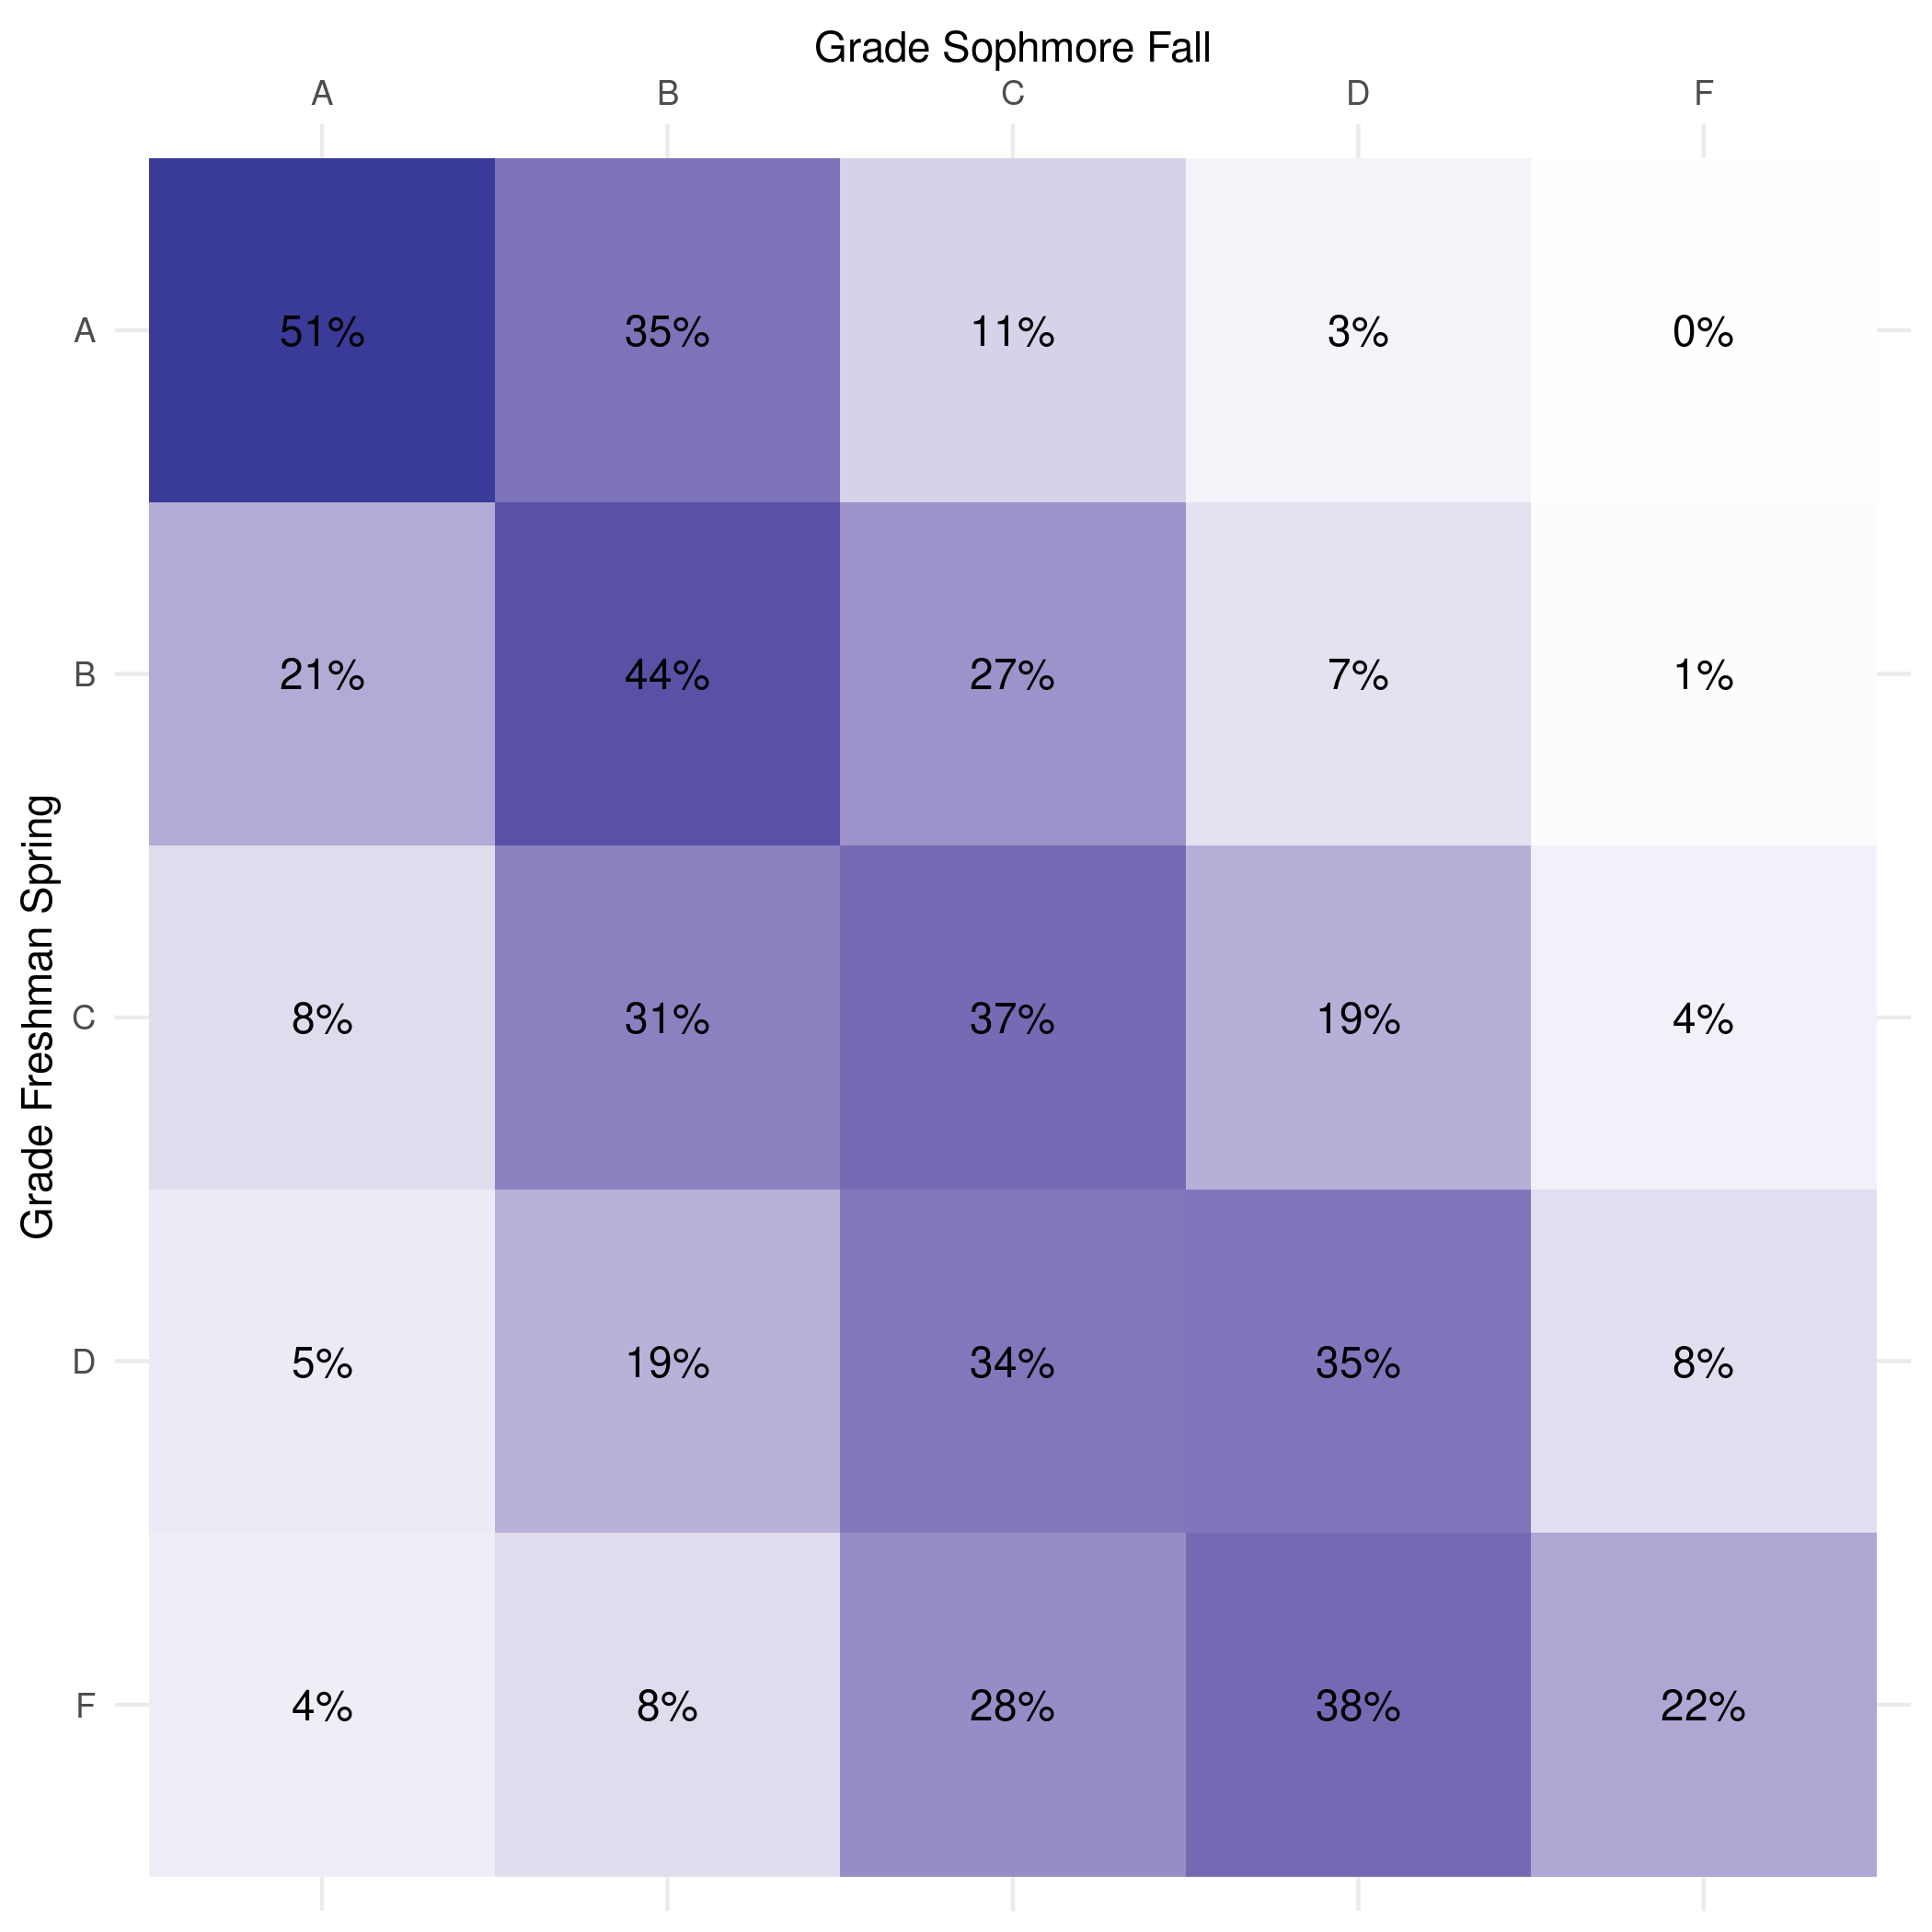
\includegraphics[width=\textwidth]{/Users/roymckenzie/Dropbox/Thesis/ECON/Output/grade_comp_math.png}
		\caption{Math Grades}
	\end{subfigure}
	\hfill
	\begin{subfigure}[b]{0.49\textwidth}
		\centering
		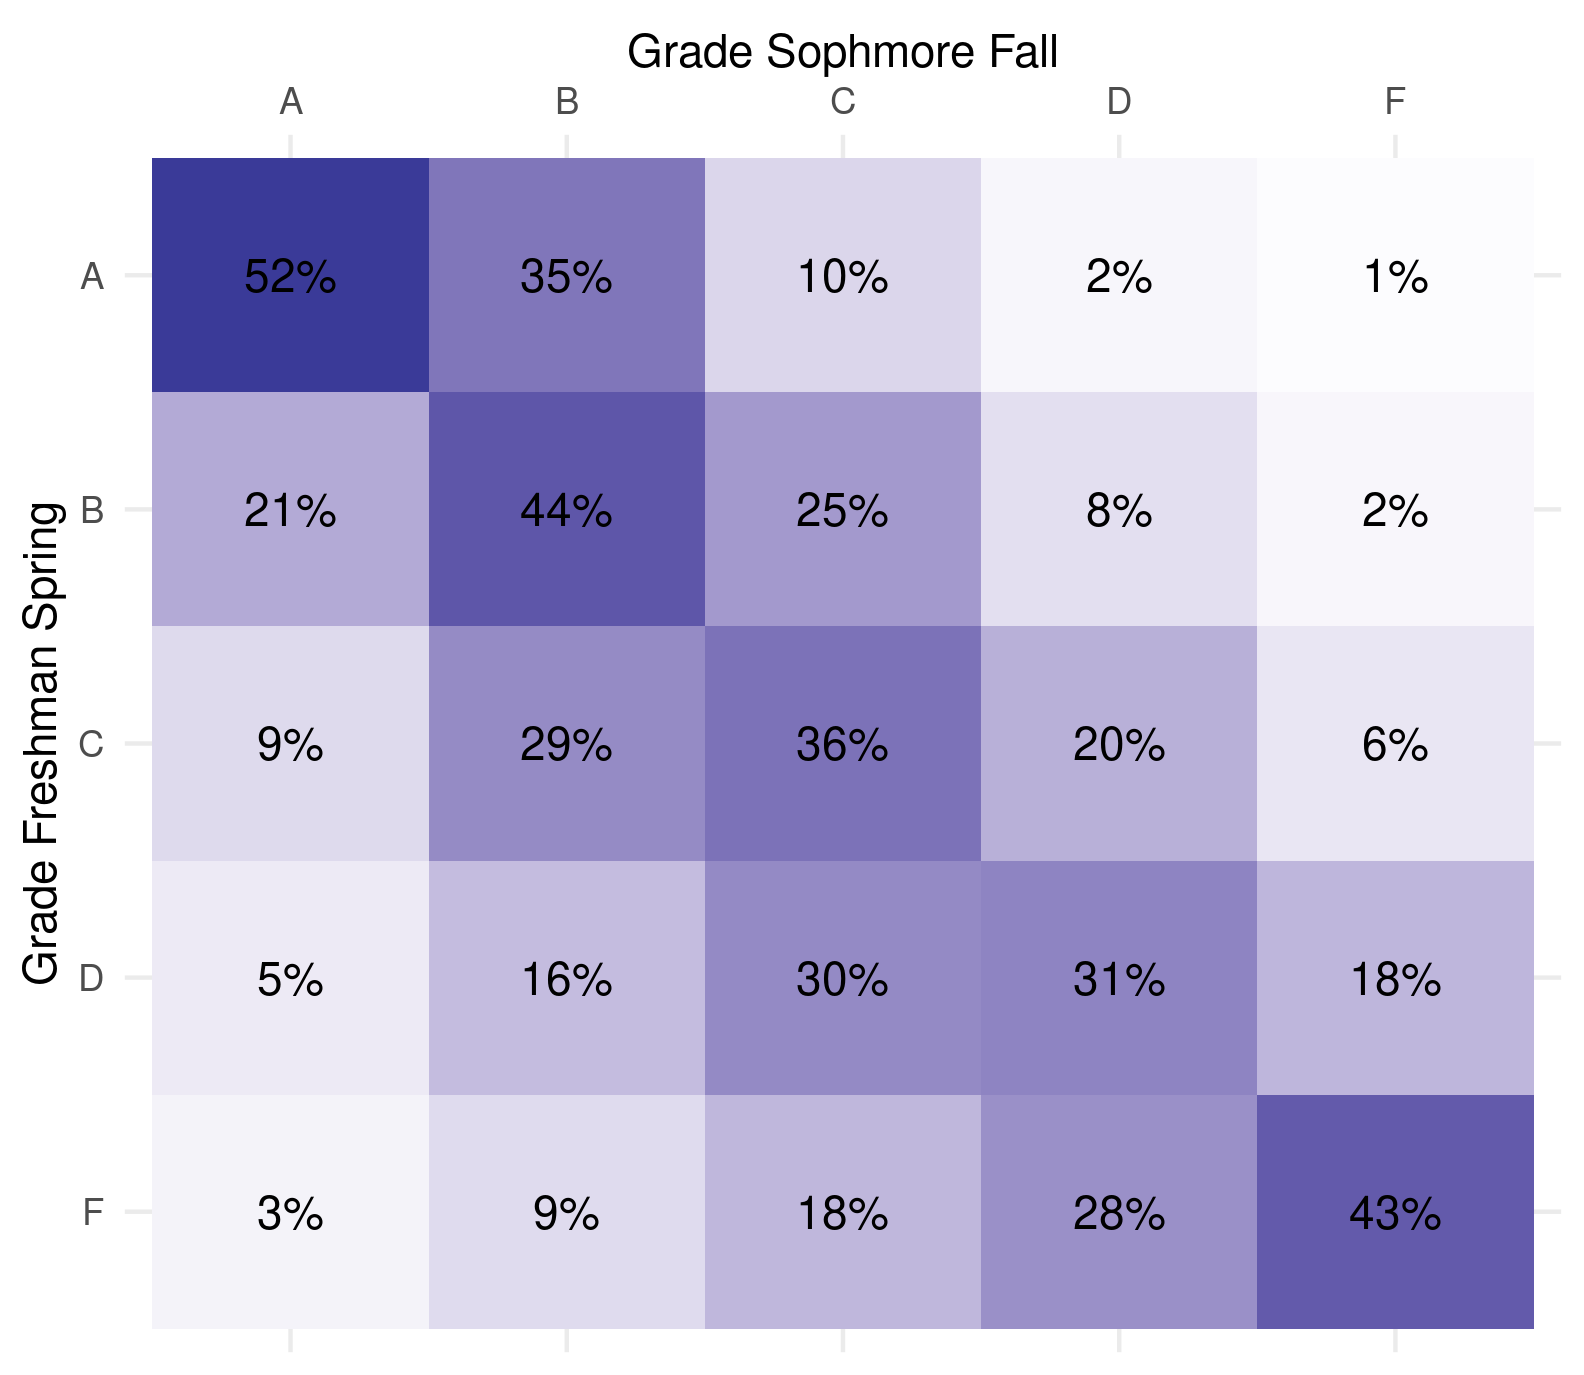
\includegraphics[width=\textwidth]{/Users/roymckenzie/Dropbox/Thesis/ECON/Output/grade_comp_eng.png}
		\caption{English Grades}
	\end{subfigure}
	\caption{Relationship Between Freshman and Sophomore Year Grades, by Subject}
	\label{fig:grade_comp}
\end{figure}

\subsection{Estimation Procedure}

\subsubsection{Estimation Procedure}

To estimate the teacher gradingg effect $\nu_j$ in the data, I  adopt a two-step method commonly used in the teacher value-added literature. First, I  follow \citet{chettyMeasuringImpactsTeachers2014} and remove observable characteristics from our grade outcomes by estimating the following equation using OLS
\begin{equation}
	g_{it}-g_{i,t+1} = \alpha_{j(it)} + \beta X_{i,t} + \varepsilon_{e_{it}}
	\label{eqn:ge_eqn}
\end{equation}
where $\alpha_{j(it)}$ represents fixed effects for teacher $j(it)$, the teacher assigned to student $i$ in period $t$. Here, $\beta_{X}$ represents a vector of student-, class-, and school-level, controls including student demographic characteristics and up to cubic terms of prior achievement, as well as classroom level means of these variables. Including the teacher fixed effects ensures that $\beta^*$, the estimate of $\beta$, is identified using only within-teacher variation, ensuring that any unobservable teacher sorting in period $t$ will not result in over-estimates of the magnitude of these grade-effects. 

Estimating the above equation returns the vector $\beta^*$, from which I  can construct a residualized grade difference, $G_{it}^*$, given as
\begin{equation}
	G_{it}^* = g_{it}-g_{i,t+1}-\beta^* X_{it}  = \alpha_{j(it)} + \varepsilon_{it}
\end{equation}
The variable $G_{it}^*$ represents the grade-difference between freshman and sophomore year for student $i$, net of any difference predicted by observable characteristics. To isolate the componenet of these residuals due to individual teacher effects, I then estimate the above as the following random intercepts model:
\begin{equation*}
	\label{eqn:re_eqn}
	G_{it^{*}} = \nu_{j(it)} +{e_{it}}
\end{equation*} 
Here, to construct empirical Bayes estimates of the grade effects, $\hat{\nu_{j(it)}}$, \citet{chettyMeasuringImpactsTeachers2014} use a jack-knifed, leave-year-out method utilizing observations for the same teacher over multiple years to estimate grade effect variance. I instead use a simple best linear unbiased predictor, or BLUP, to construct the empirical Bayes estimates of these grade effects. While I hope, in future work, to further adapt this methodology to use multiple years of teaching data, the amount of teacher turnover in CPS during the years examined, however, makes the BLUP a suitable substitute. 
%% TODO: Get a better shrinkage thing (use Raudenbush) or find a citation for BLUP or something 

%% TODO: How to get true mean?
I estimate Equation~\ref{eqn:ge_eqn} and Equation~\ref{eqn:re_eqn} separately by subject and year, and present the plot the distribution of the corresponding grade effects in Figure~\ref{fig:ge_dist} below. These effects are presented in terms of deviation from the mean per-year teacher effect, thus are artificially centered around zero. On average, the grade effects are centered closely around zero, and follow a relatively near normal distribution in shape, as is to be expected when using BLUP. 

\begin{figure}[H]
	\centering
	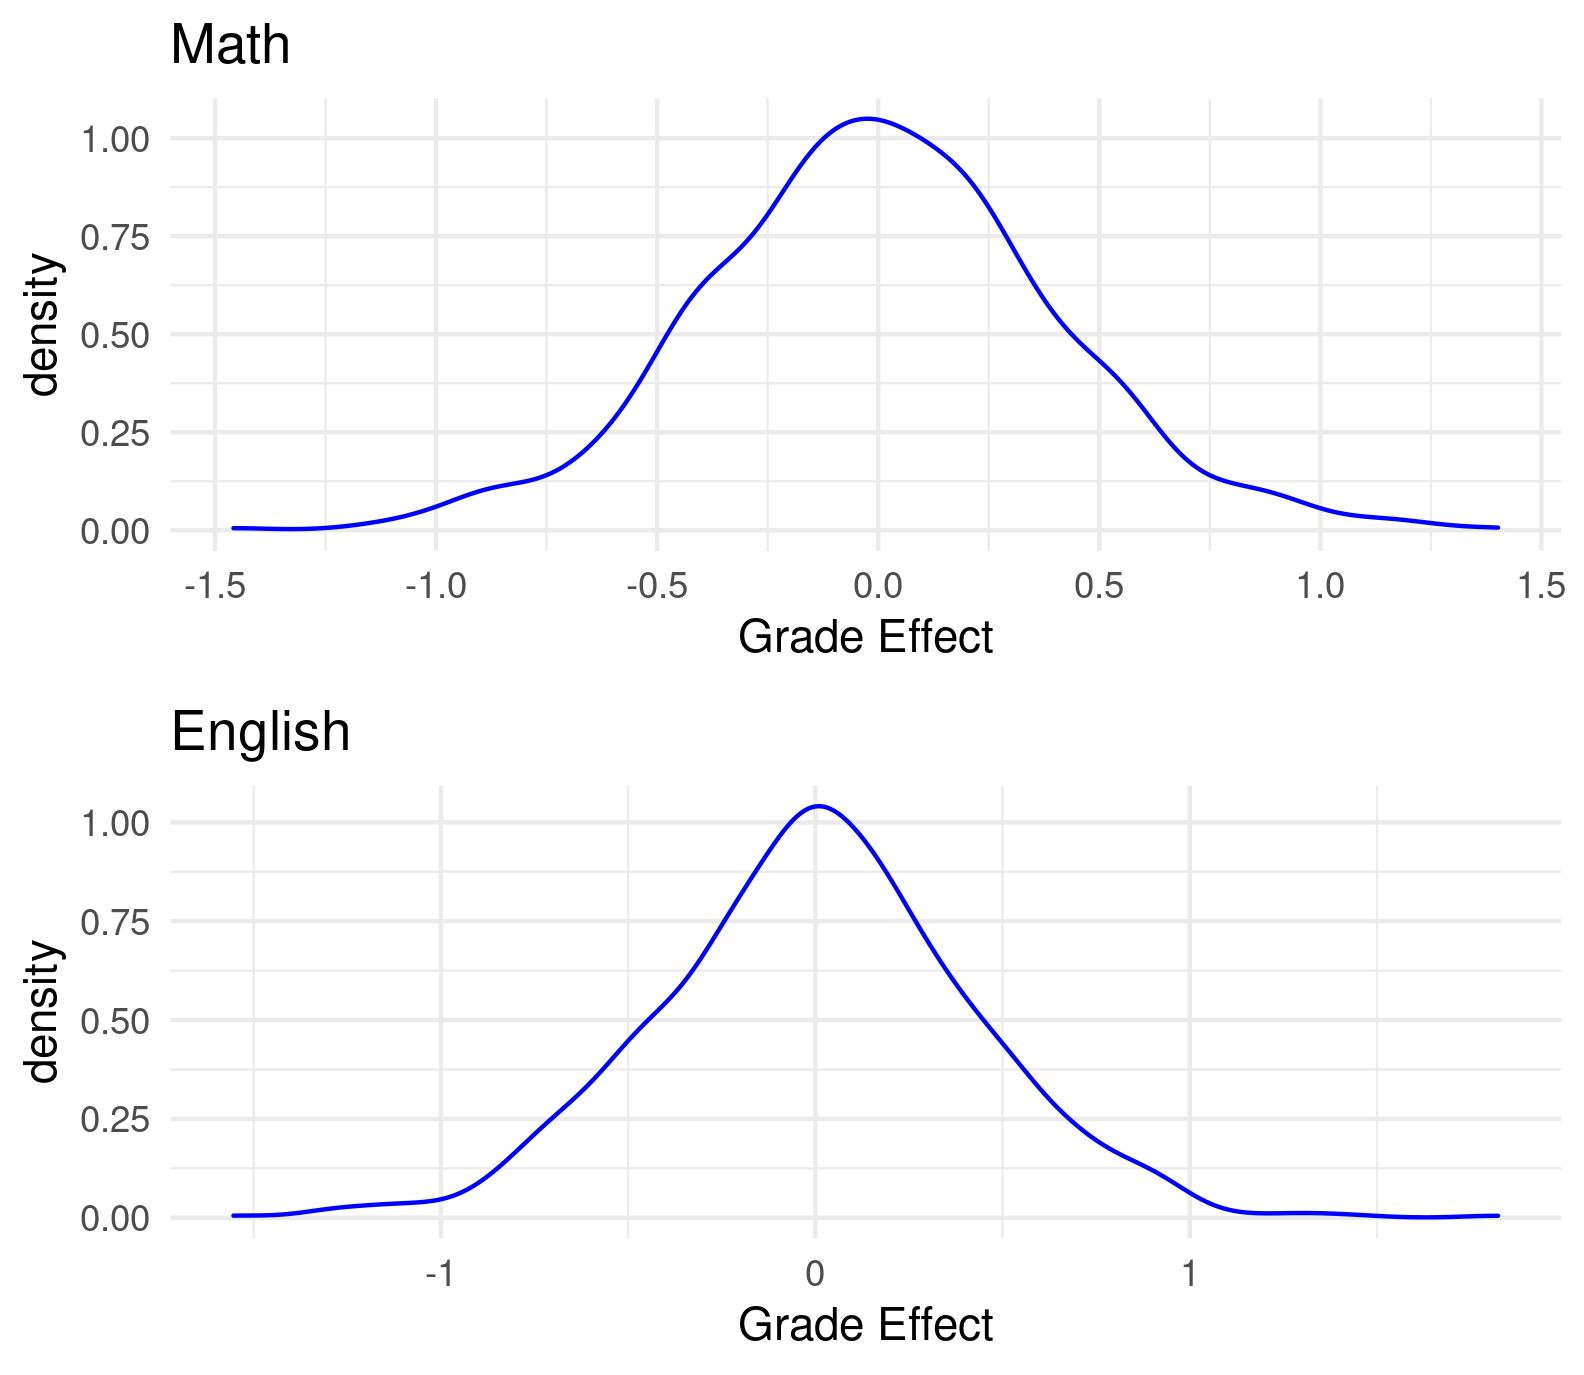
\includegraphics[width=.7\textwidth]{/Users/roymckenzie/Dropbox/Thesis/ECON/Output/Grade_Effect_Density.jpeg}
	\caption{Distribution of Estimated Grade Effects by Subject}
	\label{fig:ge_dist}
\end{figure}



\end{document}